% !TEX encoding = UTF-8
% !TEX TS-program = pdflatex
% !TEX root = ../tesi.tex

%**************************************************************
\chapter{Orchestrazione container}
\label{cap:orchestrazione-container}
%**************************************************************

\intro{Breve introduzione al capitolo}\\
In questo capitolo verrà esplicata la metodologia di orchestrazione tra container adottata in Azienda, fornendo al lettore, in primis, una panoramica su Docker Compose e, successivamente, l'integrazione dello stesso per la corretta costruzione di una \textit{sandbox} applicativa di HDA.
%**************************************************************
\section{Breve panoramica su Docker Compose}
\textbf{Docker Compose} è uno strumento per la gestione ed orchestrazione di applicazioni Docker \textbf{multi-container}. In un ambiente costituito da multipli container in esecuzione, può essere relativamente \textbf{difficile} e \textbf{gravoso} per l'utente manutenzionare, avviare o fermare multipli container. Per aiutare appunto nell'orchestrazione, intesa come \textbf{monitoraggio}, \textbf{avvio}, \textbf{ri-avvio} in caso di \textit{failure} ed \textbf{arresto} di multipli container, l'utente può installare Docker Compose sulla propria workstation, per centralizzare così la gestione di tutti i container da un'unica interfaccia.\\
Tramite definizione di un file \textbf{YAML} (ex: \textit{docker-compose.yml}), si può istruire Docker Compose relativamente a quali container dovrà avviare specificando, inoltre, eventuali parametri aggiuntivi, quali \textit{volume-mapping} o interfacce di rete aggiuntive.\\
I passi che Docker Compose esegue per creare quindi la \textit{sandbox} applicativa di HDA sono i seguenti:
\begin{itemize}
	\item \textbf{lettura} del file docker-compose.yml;
	\item lettura, ricorsiva, dei \textbf{dockerfile} relativi ai \textbf{container} definiti nel docker-compose.yml;
	\item \textbf{costruzione}, secondo l'ordine ed eventuali parametri definiti nel docker-compose.yml, delle \textbf{immagini} dei container dichiarati nel Compose-file (docker-compose.yml).
\end{itemize}
Una volta costruite tutte le immagini dei container propri della \textit{sandbox} applicativa di HDA, è possibile lanciare la \textit{sandbox} applicativa tramite il semplice comando: \centerline{\textbf{docker-compose
-f docker-compose.yml -p nomecliente up}} sostituendo "nomecliente" con il nome effettivo del cliente \textbf{proprietario} della \textit{sandbox} di HDA. I parametri \textbf{-f} e \textbf{-p} definiscono, rispettivamente, la possibilità di dichiarare un Compose-file alternativo e la possibilità di assegnare un nome alternativo all'istanza, la quale, di \textit{default}, acquisirebbe il nome della directory contenente il Compose-file.

%\label{sec:tecnologie-strumenti}

%\subsection*{Tecnologia 1}
%Descrizione Tecnologia 1.

%**************************************************************
\section{Docker compose per la costruzione di una sandbox applicativa}
Come visto nel paragrafo precedente, tramite Docker Compose è possibile orchestrare l'avvio e l'arresto di una intera \textit{sandbox} applicativa di HDA tramite un \textbf{singolo comando}. Tramite l'uso di Docker Compose, l'esecuzione \textbf{simultanea} di più \textit{sandbox} applicative di HDA risulta di semplice esecuzione, in quanto basterà lanciare nuovamente il comando descritto nel paragrafo precedente per creare una nuova \textit{sandbox} applicativa destinata ad un altro cliente. \\
Ogni \textit{sanbdbox} ha un nome, il quale deve necessariamente essere \textbf{univoco}.
La seguente immagine mostra una panoramica, fornita da Docker Compose, di due \textit{sandbox} applicative, con i relativi container di cui composte, in esecuzione \textbf{simultanea} sullo stesso \textit{host}, chiamate rispettivamente \textit{nomecliente} e \textit{cliente2}:
\begin{figure}[!h]     
\centering 
    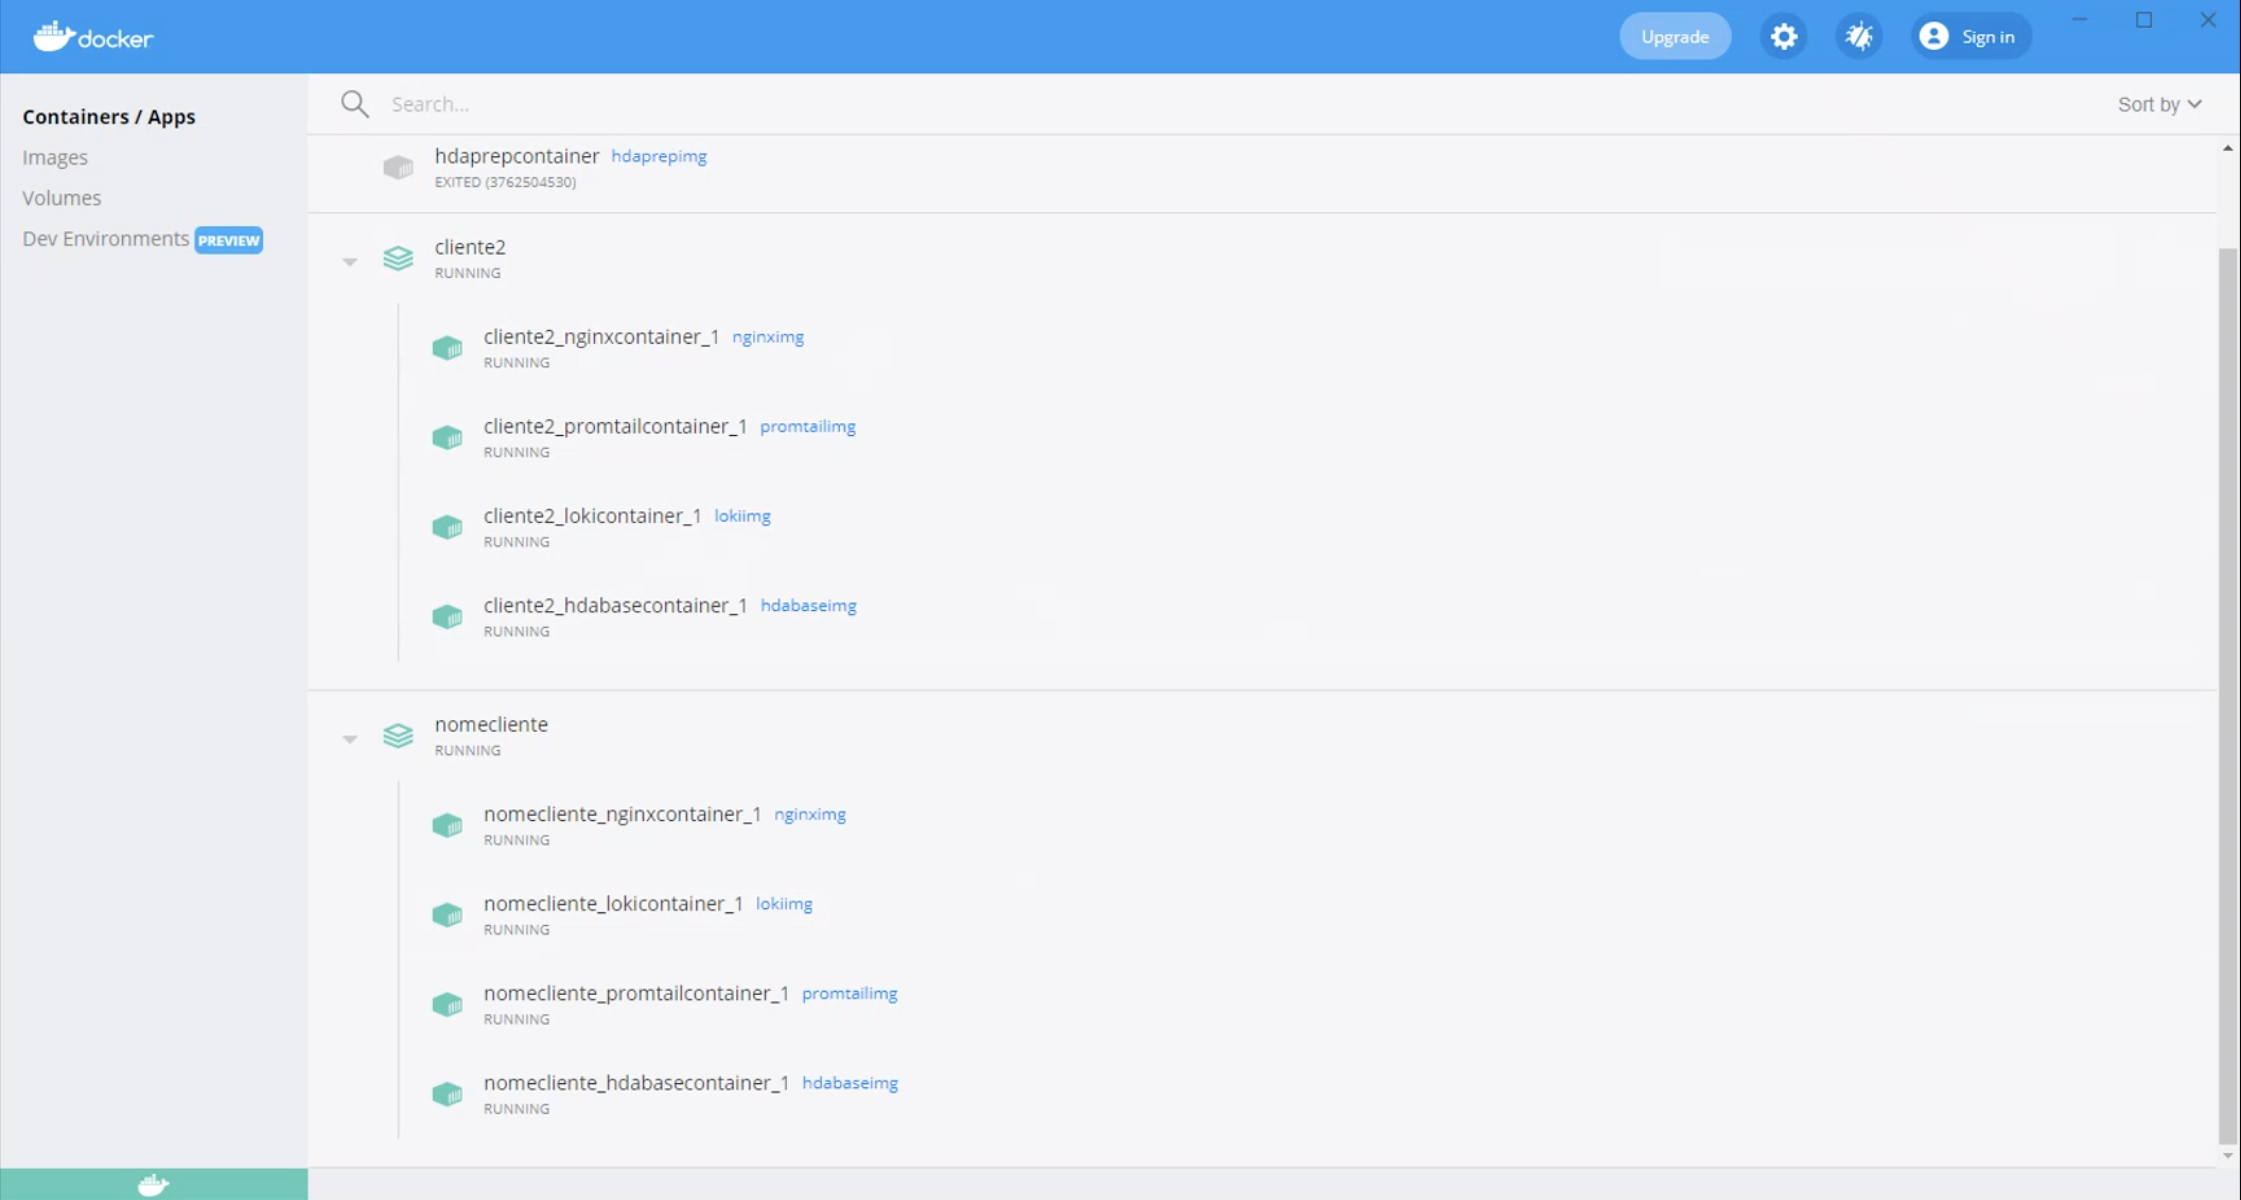
\includegraphics[width=1.0\columnwidth]{immagini/screenshot/docker_compose_sandbox} 
    \caption{Interfaccia di Docker Compose con in esecuzione due \textit{sandbox} applicative}
\end{figure} \\
%\subsubsection{Namespace 1} %**************************
%Descrizione namespace 1.


%**************************************************************
\section{Integrazione di HDA Sandbox Builder con Docker Compose}
Come visto all'interno di questo capitolo, tramite Docker Compose è possibile la costruzione delle immagini relative ai container che comporranno, successivamente, una volta lanciati in esecuzione, la \textit{sandbox} applicativa di HDA. Per arrivare ad una corretta esecuzione di una \textit{sandbox} applicativa però, la costruzione tramite Docker Compose dei container stessi che la compongono \textbf{non è sufficiente}. E' il caso, ad esempio, del container atto alla preparazione del filesystem di HDA ("hdaprepcontainer"), senza il quale l'istanza di HDA \textbf{non riuscirà ad avviarsi} a causa di un \textit{settaggio} errato dei permessi nella cartella \textbf{/App\_Data} dello stesso. Questo container non è inserito all'interno all'interno del Compose-file, in quanto deve essere \textbf{manualmente lanciato e supervisionato} dall'utente installatore, e l'esecuzione del container dovrà terminare \textbf{prima} di poter lanciare una qualsiasi \textit{sandbox} applicativa di HDA. Anche il container "hdadbupdatercontainer" è escluso dal Compose-file, in quanto, anch'esso, dovrà essere \textbf{eseguito manualmente} dall'utente installatore e continuamente supervisionato durante la sua completa esecuzione.\\
E' quindi facilmente intuibile, che l'esecuzione di Docker Compose dovrà essere necessariamente \textbf{subordinata} all'esecuzione del \textit{batch-file} \textbf{HDA\_sandbox\_builder.bat}.\\
Riassumendo, i passi atti ad una corretta esecuzione di una \textit{sandbox} applicativa di HDA sono i seguenti:
\begin{itemize}
	\item \textbf{Passo 1:} lancio del \textit{batch-file} \textbf{HDA\_sandbox\_builder.bat}, con costruzione ed esecuzione \textbf{obbligatoria} del container "hdaprepcontainer";
	\item \textbf{Passo 2:} creazione di una directory avente nome del cliente stesso che conterrà il \textit{filesystem} della nuova \textit{sandbox} applicativa di HDA generato dal passo precedente;
	\item \textbf{Passo 3:} da prompt dei comandi con privilegi di amministratore, lanciare il comando "\textbf{xcopy}" relativamente ai file situati nella cartella App\_Data del container "hdaprepcontainer", situato all'interno della directory creata al punto precedente;
	\item \textbf{Passo 4:} esecuzione del comando di Docker Compose "\textbf{docker-compose-f docker-compose.yml -p nomecliente up}" sostituendo al posto della stringa "nomecliente" il \textbf{nome del cliente scelto} nel passo 2.
\end{itemize}
L'obbligatorietà dell'esecuzione manuale di questi quattro distinti passi è stata \textbf{strettamente voluta dall'Azienda}, in quanto ha preferito non automatizzare l'intera procedura di creazione di una \textit{sandbox} applicativa per avere un maggior controllo in ogni "passo" della sua creazione.\\
Il corretto instradamento degli accessi da parte degli utenti alle istanze di HDA contenuta nel relativo container ("hdabasecontainer") all'interno delle \textit{sandbox} applicative sarà trattato nel prossimo capitolo.







%**************************************************************